\section{Background}

In this section, we present some of design basics of FAT file system and NTFS file system, 
which are relevant to what we discuss in the latter part of the paper. 
We highlight what information remains in the file system after a file is deleted, 
which leads to understanding of how metadata-based file-recovery might work. 
Finally, we briefly present NIST standards for such recovery tools.  

\subsection{FAT Filesystem}

The role of metadata and actual content of a file in FAT filesystem is illustrated with an example file in Figure~\ref{fig:fat1}.

\begin{figure}[h]
    \centering
    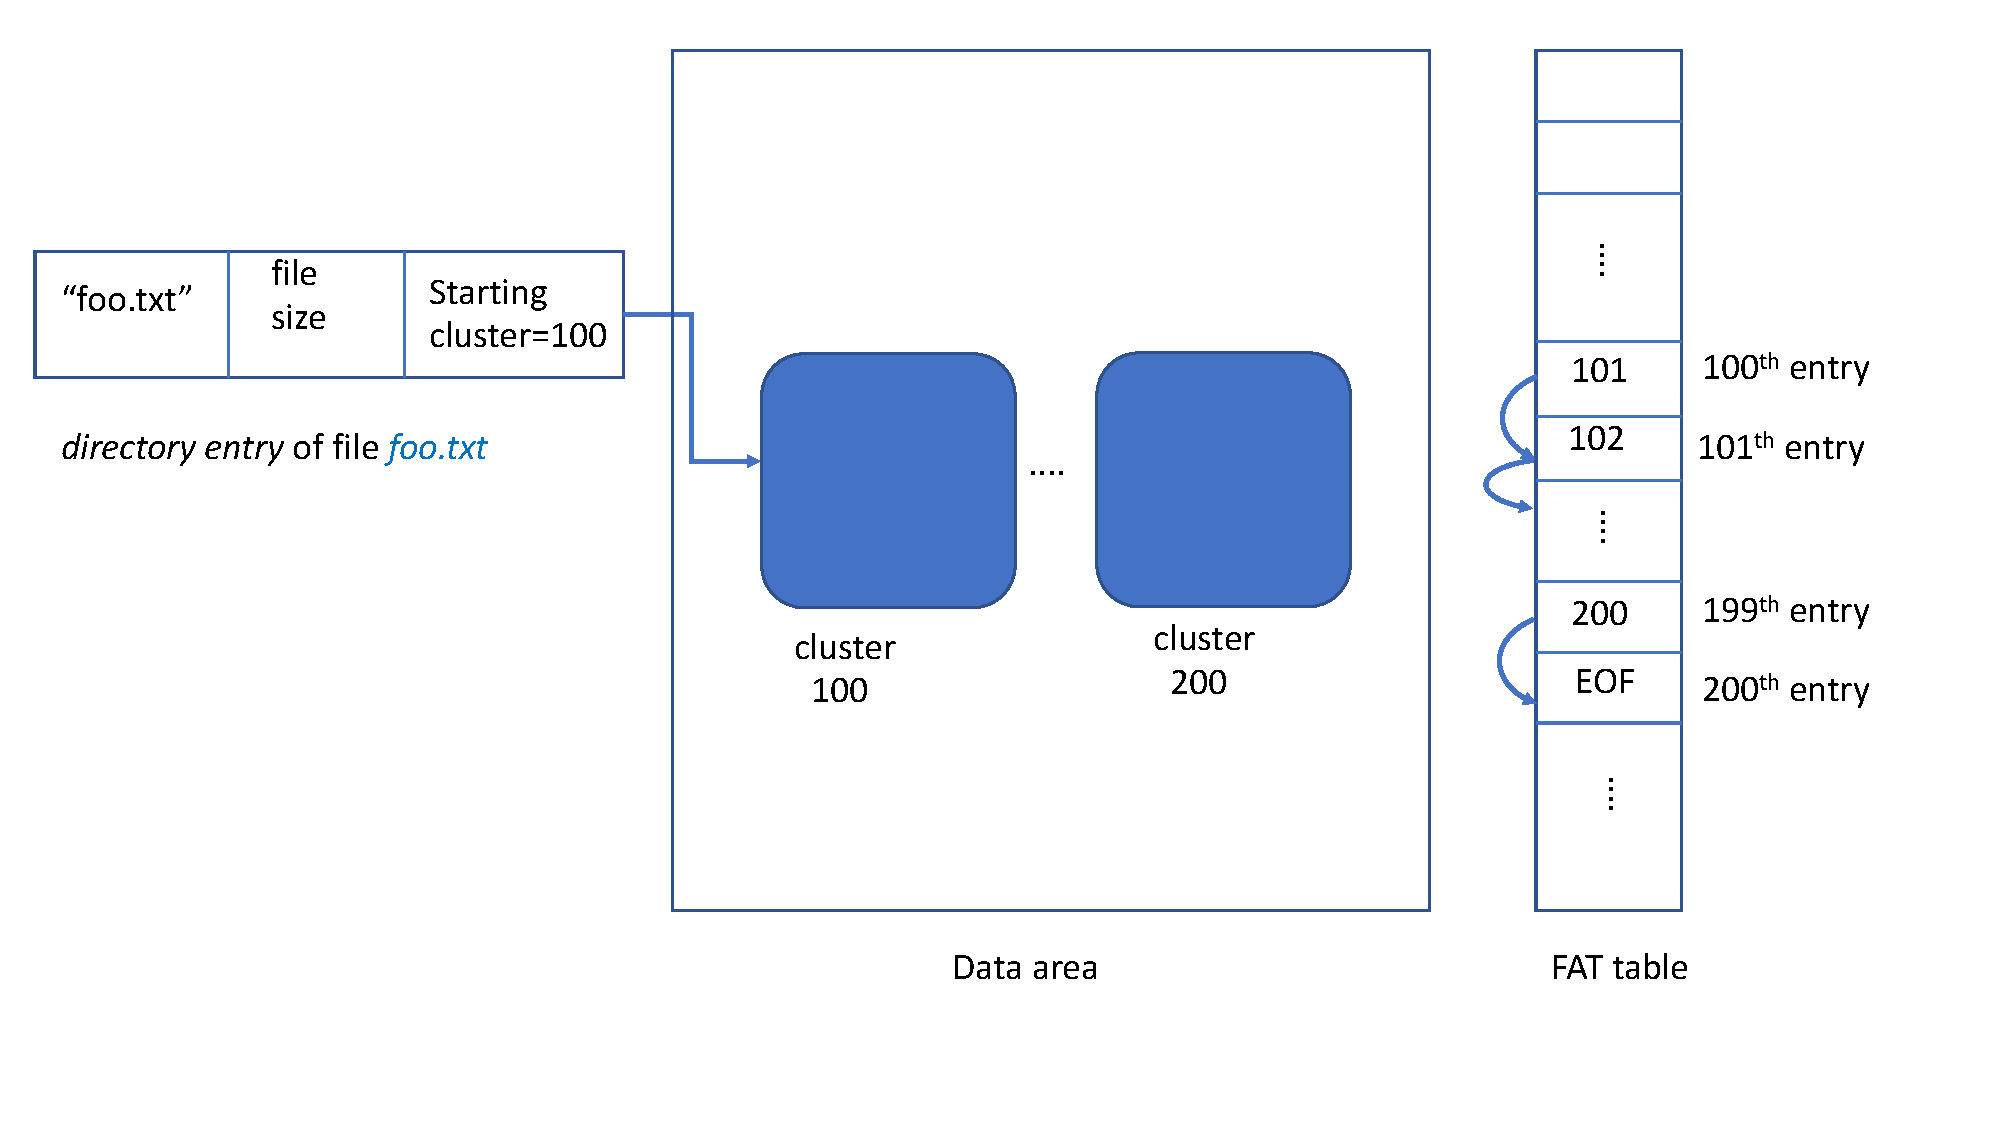
\includegraphics[width=\linewidth]{fig/fat1.pdf}
    \caption{The role of metadata and actual content of a file foo.txt in FAT filesystem is shown. FAT table is also drawn.}
    \label{fig:fat1}
\end{figure}


The change in metadata and actual content of foo.txt is illustrated in Figure~\ref{fig:fat2} when the file is deleted.

\begin{figure}[h]
    \centering
    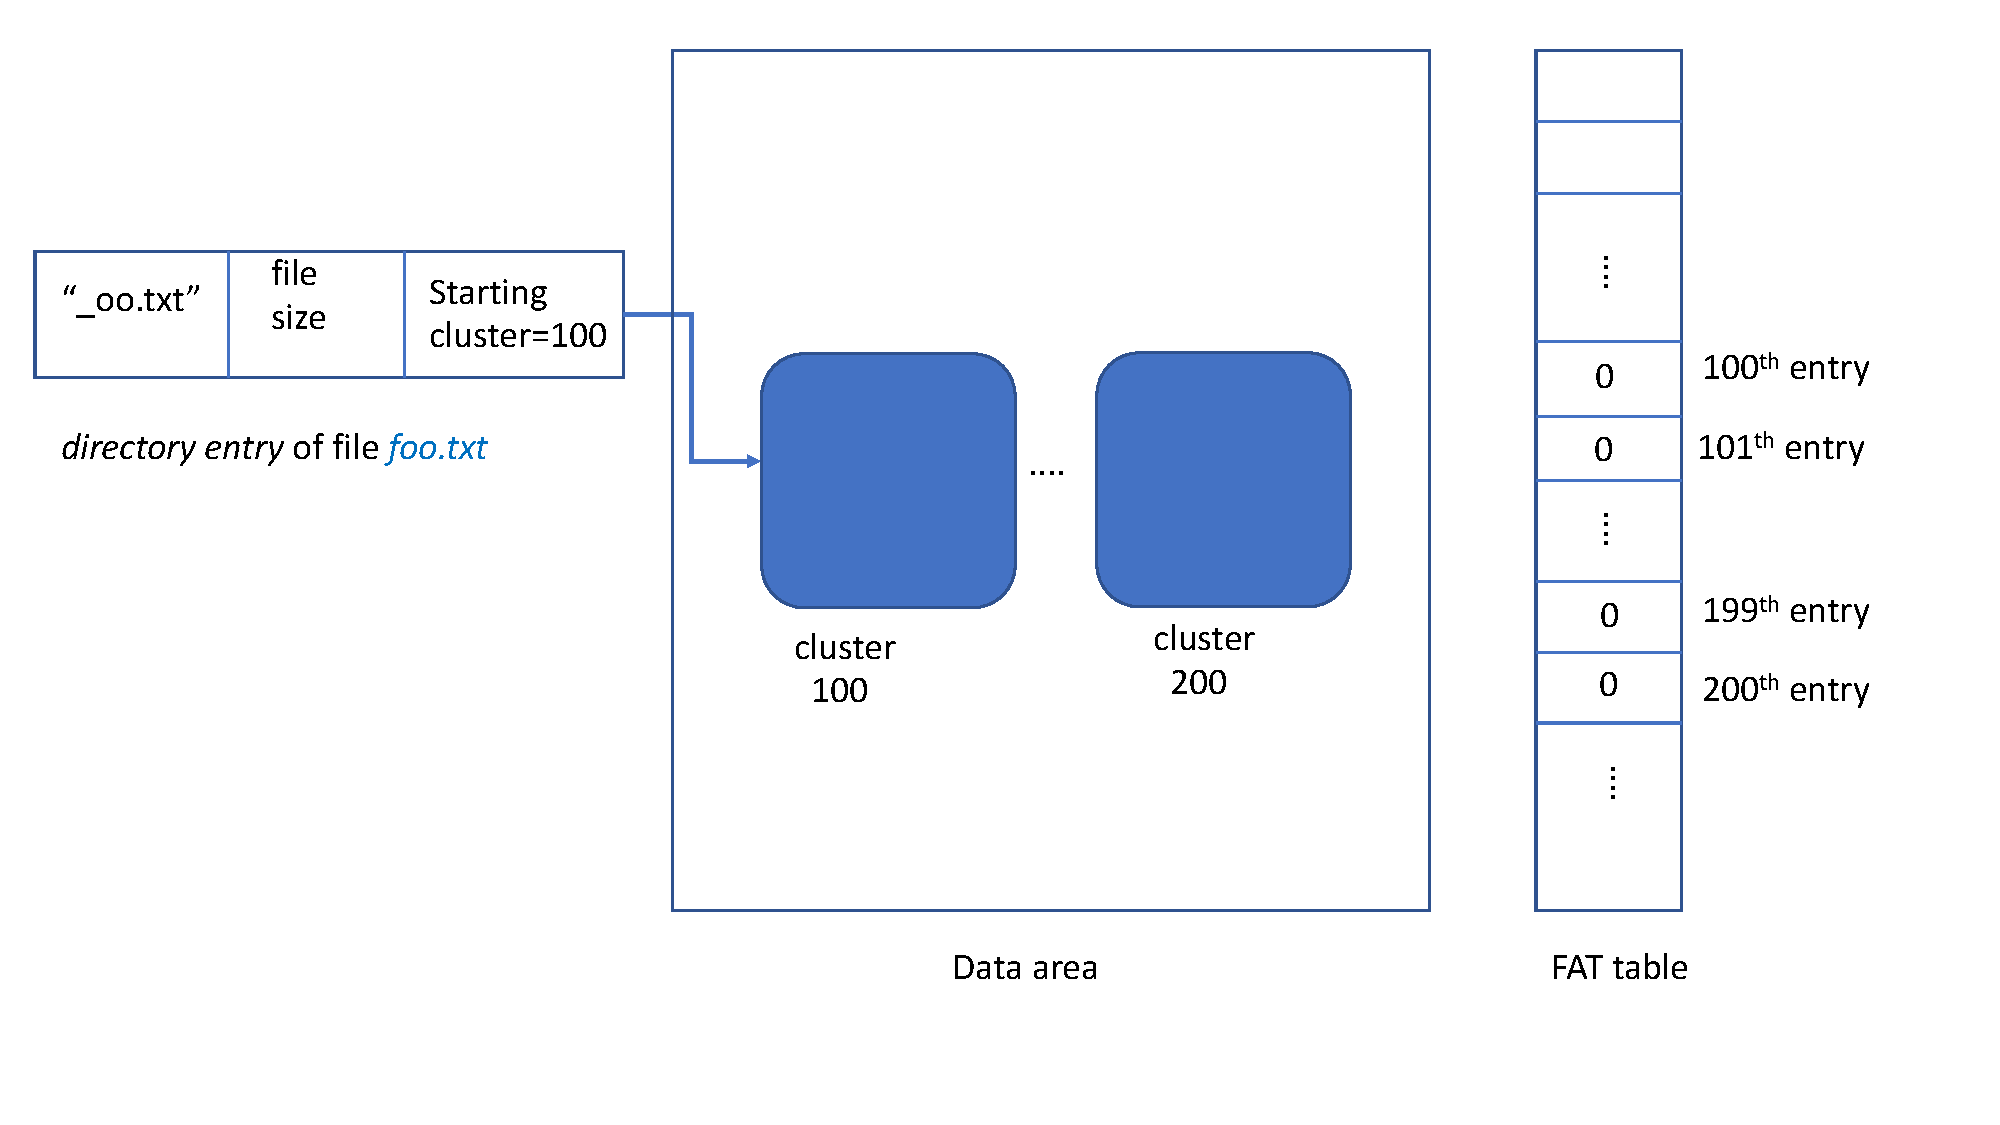
\includegraphics[width=\linewidth]{fig/fat2.pdf}
    \caption{The change in metadata and actual content of foo.txt is shown when the file is deleted. FAT table is also drawn.}
    \label{fig:fat2}
\end{figure}

Furthermore, it is possible that the content of a file is not stored in contiguous clusters in FAT filesystem. 
If the orginal file foo.txt has two fragments, it may look as illustrated in Figure~\ref{fig:fat3}.

\begin{figure}[h]
    \centering
    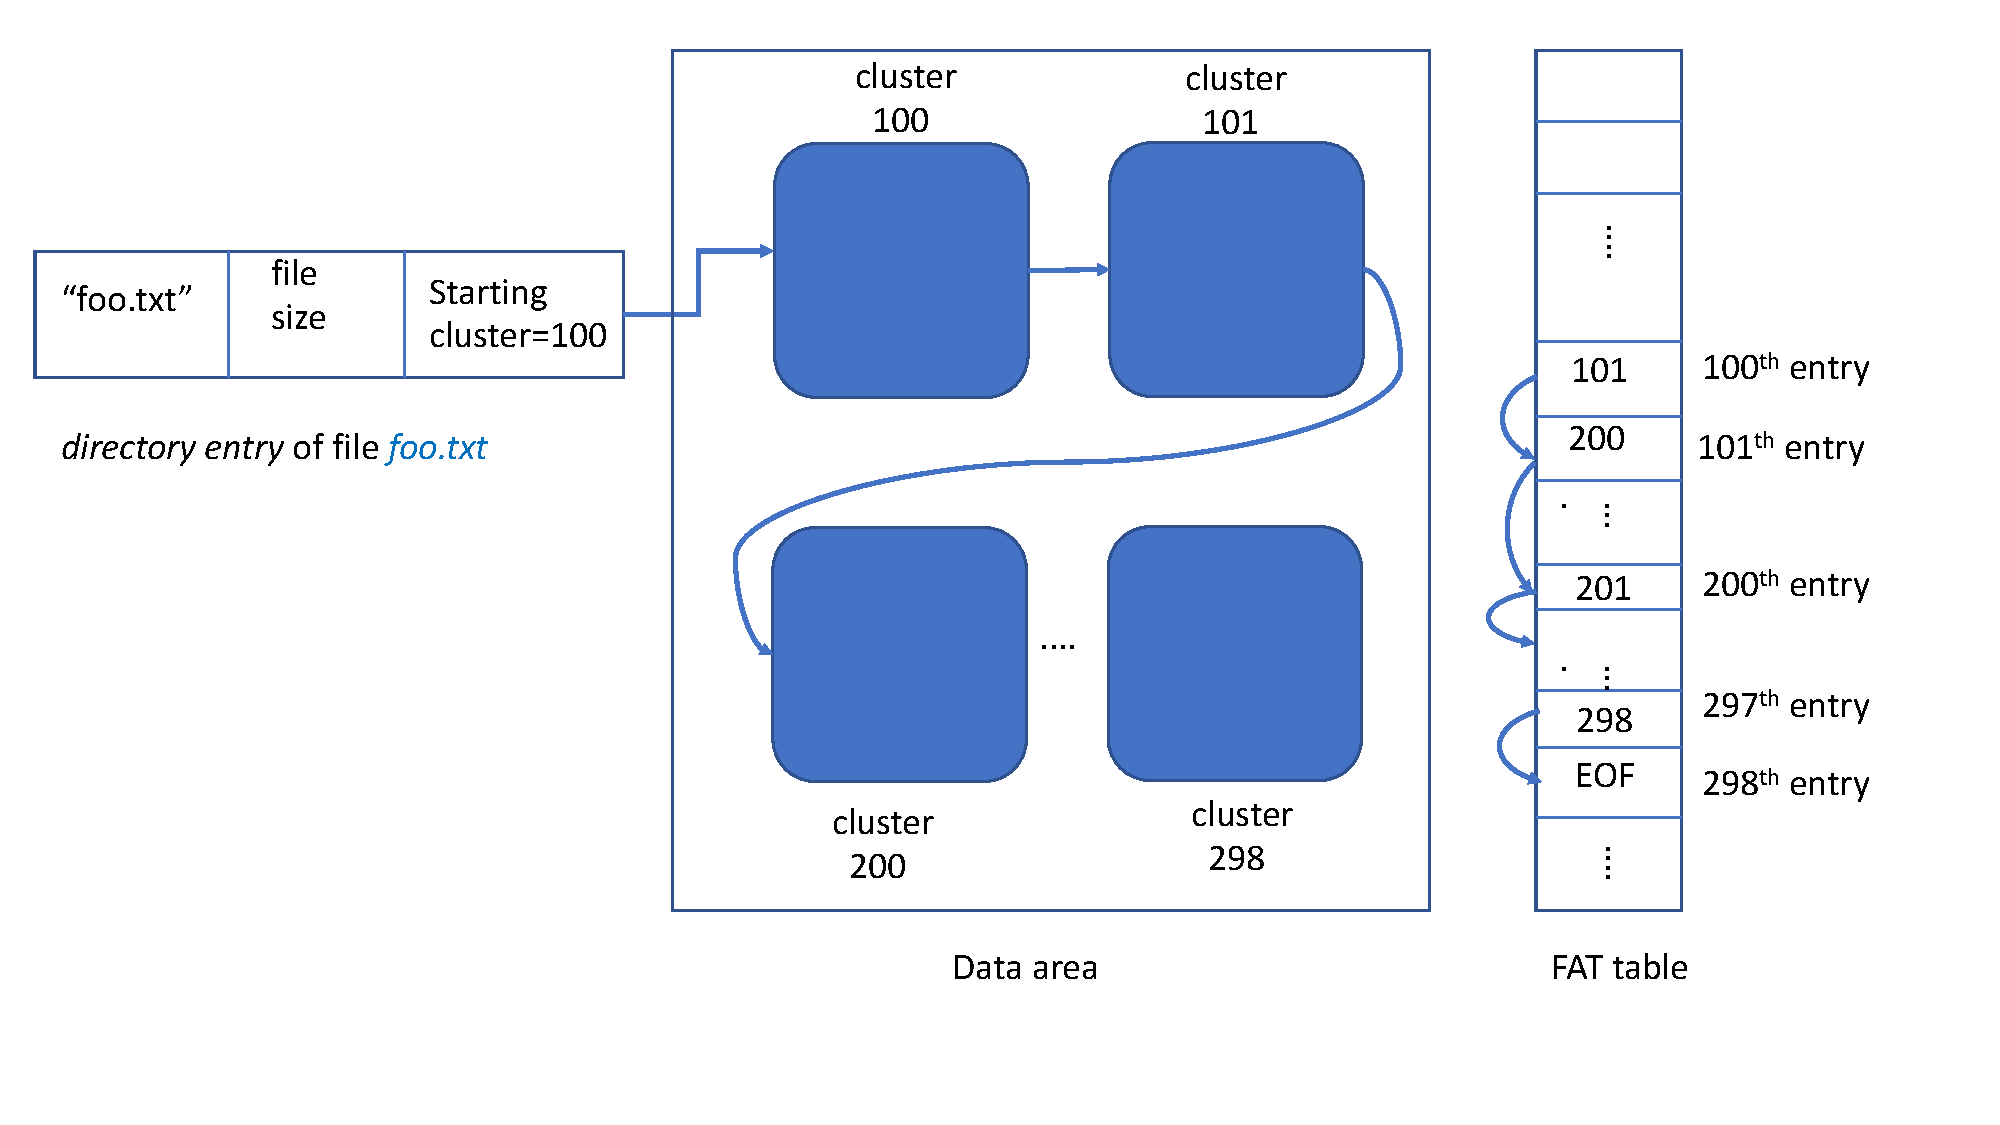
\includegraphics[width=\linewidth]{fig/fat3.pdf}
    \caption{The role of metadata and actual content of a file foo.txt is shown whereas the file has two fragments. FAT table is also drawn.}
    \label{fig:fat3}
\end{figure}
\subsection{NTFS Filesystem}

The role of metadata and actual content of a file in NTFS filesystem is illustrated with an example file in Figure~\ref{fig:ntfs}.

\begin{figure}[h]
    \centering
    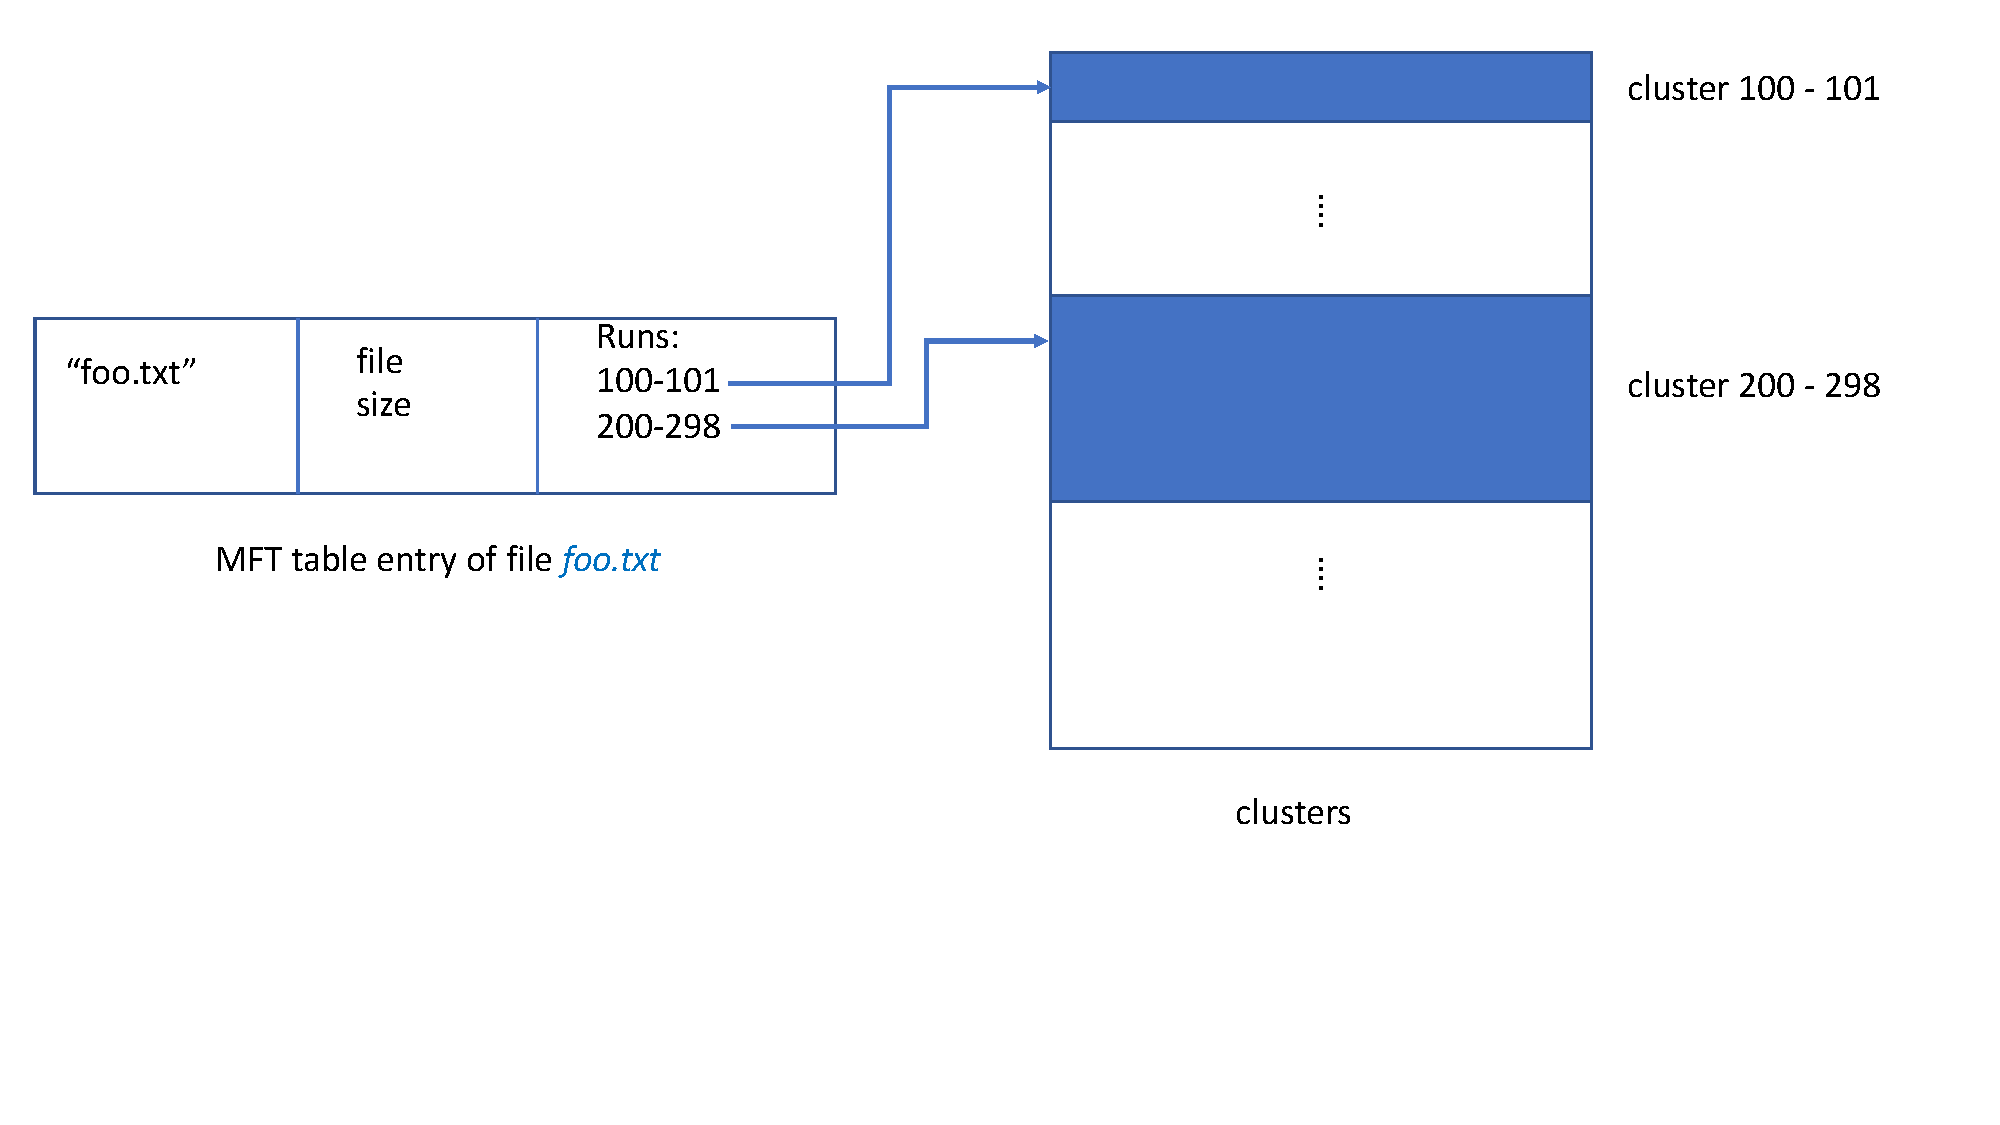
\includegraphics[width=\linewidth]{fig/ntfs.pdf}
    \caption{The role of metadata and actual content of a file foo.txt in NTFS filesystem is shown. MFT table entry of the file as well as data containing clusters are shown.}
    \label{fig:ntfs}
\end{figure}
\subsection{Metadata-Based Deleted File Recovery}

\subsection{NIST Standards}
\begin{enumerate}
 \item ``The tool shall identify all deleted File System-Object entries accessible in residual metadata.''\cite{meta:dfr:standards}
 We consider a tool passing this standard if it identifies to the user each filesystem metadata entry that is marked as deleted.
 \item ``The tool shall construct a Recovered Object for each deleted File System-Object entry accessible in residual metadata.''\cite{meta:dfr:standards}
 We consider a tool passing this standard as long as it outputs a file for each deleted file, even if the output file is empty.
 \item ``Each Recovered Object shall include all non-allocated data blocks identified in a residual metadata entry.''\cite{meta:dfr:standards}
 For FAT filesystems, we consider a tool passing this standard if it recovers at least the first contiguous segment of unallocated sectors starting from the first sector originally allocated to the deleted file. For NTFS filesystem, the tool must recover all unallocated sectors originally allocated to the deleted file.
 \item ``Each Recovered Object shall consist only of data blocks from the Deleted Block Pool.''\cite{meta:dfr:standards}
 We consider a tool passing this standard if the recovered file consists only of data from the original deleted file, or null data to represent omitted portions.
\end{enumerate}


